\subsection{Regime superfluido}% foto
\begin{frame}{Regime superfluido}
  Interazioni $\Rightarrow$ effetti collettivi del sistema\\
    \fbox{
        \movie[%borderwidth=.6pt,
      height=5pt,
      width=5pt,
      externalviewer,	
      poster]
      {}{movies/ToSuper-exp.mov}
      }
      Regime subsonico: superfluidità\\
  \begin{columns}[t]
  
    \begin{column}{.7\textwidth}
     \begin{figure}
  \centering
    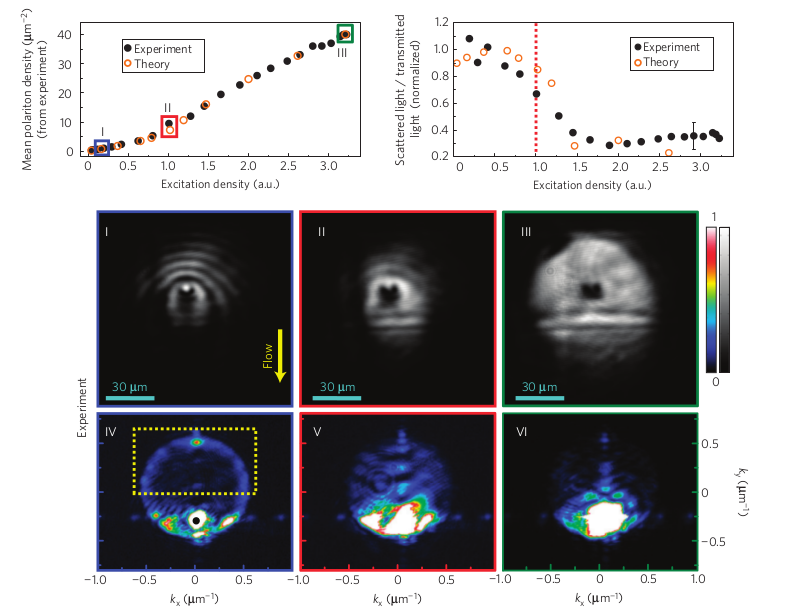
\includegraphics[width=\columnwidth]{pics/scattering-super-all.png}
  \end{figure}
  \hspace{-10pt}
    \end{column}
    \begin{column}{.3\textwidth}
    
    \begin{figure}
          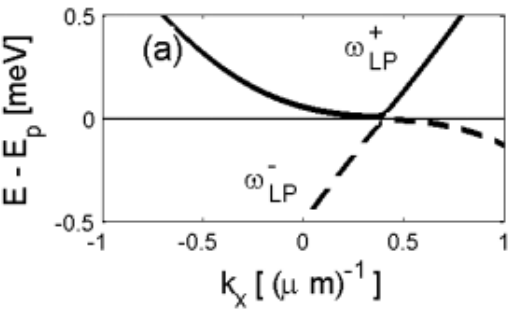
\includegraphics[width=\columnwidth]{pics/scattering-super-dispersion.png}
      \end{figure}
      Criterio di Landau
\begin{flalign*}
       \displaystyle v_p < v_{cr}\equiv \min_k \frac{\omega\bog (k)}{k}&&
\end{flalign*}
    \end{column}
  \end{columns}
\vspace{-15pt}
\scriptsize
Nota: La velocità critica di Landau definisce una ``velocità del suono" solo per $\Delta_p =0$\\
$ \qquad c_s \equiv \sqrt{\dfrac{\hbar g\lp |\psi\sts|^2}{m\lp}}$
\end{frame}

\subsection{Regime \v{C}erenkov}% foto

\begin{frame}{Regime \v{C}erenkov}
  Interazioni $\Rightarrow$ effetti collettivi del sistema\\
   \fbox{
        \movie[%borderwidth=.6pt,
      height=5pt,
      width=5pt,
      externalviewer,	
      poster]
      {}{movies/ToCher-exp.mov}
      }
      Regime supersonico: emissione \v{C}erenkov\\
  \begin{columns}[t]
  
    \begin{column}{.7\textwidth}
     \begin{figure}
  \centering
    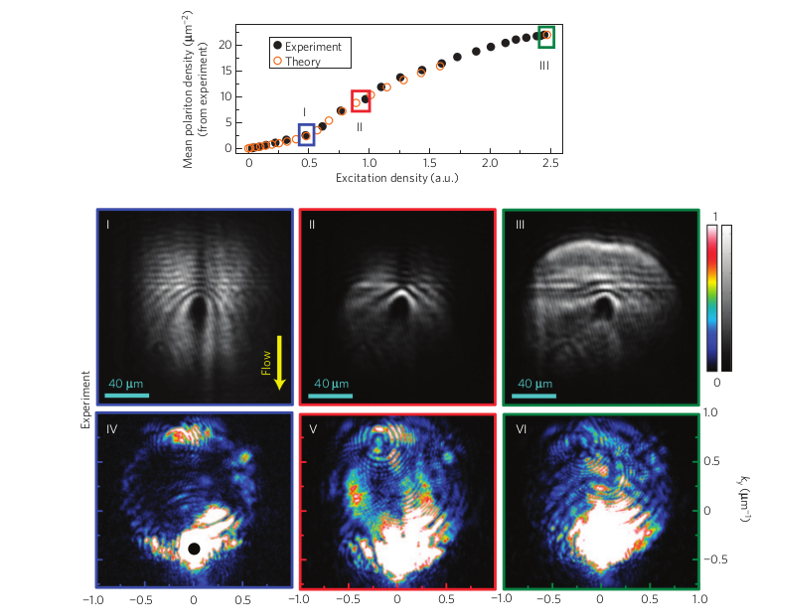
\includegraphics[width=\columnwidth]{pics/scattering-cher-all.png}
  \end{figure}
  \hspace{-10pt}
    \end{column}
    \begin{column}{.3\textwidth}
    
    \begin{figure}
          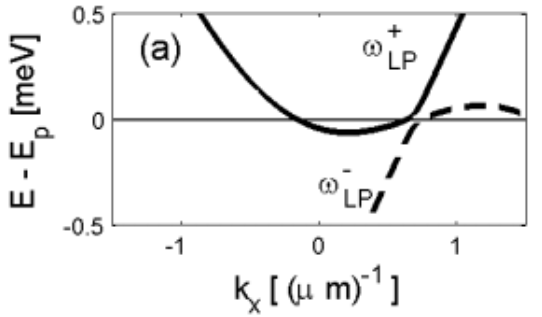
\includegraphics[width=\columnwidth]{pics/scattering-cher-dispersion.png}
      \end{figure}
      Criterio di Landau
\begin{flalign*}
       \displaystyle v_p > v_{cr}\equiv \min_k \frac{\omega\bog (k)}{k}&&
\end{flalign*}
    \end{column}
  \end{columns}
\vspace{-15pt}
\scriptsize
Nota: La velocità critica di Landau definisce una ``velocità del suono" solo per $\Delta_p =0$\\
$ \qquad c_s \equiv \sqrt{\dfrac{\hbar g\lp |\psi\sts|^2}{m\lp}}$
\end{frame}